\chapter{LSST}
\label{chapter:future}

\begin{abstract}
The Large Synoptic Survey Telescope (\LSST) will provide sparse but precise
ground-based photometry for billions of field and cluster cool dwarfs.
We explore the potential of \LSST\ for large-scale rotation period measurement
with an emphasis on applications to gyrochronology, the method of inferring
stellar ages from rotation periods.
With its ten year baseline, \LSST\ light curves will be sensitive to long
rotation periods which are characteristic of old and low-mass stars.
New asteroseismic data from the \kepler\ spacecraft have revealed that
magnetic braking may cease at around Solar Rossby number, implying that
gyrochronology is not applicable to old stars.
By measuring rotation periods of old, slowly rotating, low-mass stars we can
decisively test the age-rotation relations at all ages.
Of particular interest are the open clusters with precisely measured
isochronal ages.
These clusters will allow us to recalibrate the age-rotation relations in the
old, low-mass regime, provided we can measure the photometric rotation periods
of their members.
Using representative distributions of stellar ages and spectral types from
\TRILEGAL\ outputs, we simulated thousands of light curves using a
gyrochronology relation, a simple star-spot model and approximate \LSST\
cadence.
By running a rotation period recovery pipeline, we predict the number of
accurately measured cool dwarf rotation periods expected from \LSST\ as a
function of spectral type, magnitude and rotation period.
Using the full ten-year data set we are able to accurately recover 60-70\% of
rotation periods for stars with $T_{\mathrm{eff}}>4500$ K and 70-80\% for
stars with $T_{\mathrm{eff}}<4500$ K, brighter than 23rd magnitude.

\end{abstract}

\section{Introduction}

This project was motivated by a call for community input on the optical and
infrared follow-up requirements for stellar rotation and magnetism studies
with \LSST.
This work was undertaken in collaboration with others, however most of the
analysis was performed by myself.
Exceptions are clearly indicated in the text.

The Large Synoptic Survey Satellite (\LSST) is a 8.4 metre telescope with a
9.6 square degree field of view in Cerro Pach\'{o}n, Chile, currently under
construction.
It is designed to observe 18,000 square degrees in the southern sky (south of
+10 degrees, declination) in six Sloan Digital Sky Survey (\SDSS) filters:
{\it ugrizy}.
During its main mode of operation (90\% of the time), \LSST\ will perform two
fifteen second exposures per visit, with one thousand visits per night and
will have a faint limit of around 24.5 in r-band.
For the remaining 10\% of the time, \LSST\ will focus on a small number of
`deep drilling fields'.
These fields are yet to be determined but could be, for example, the Large and
Small Magellanic Clouds, the galactic plane, and so on.
These fields will receive targeted, repeat observations of, for instance 200
observations over a 40-hour period after which the faint limit could be
extended to around 28 apparent magnitudes.
First light is currently scheduled for 2021 and data release one of eleven is
expected to contain eighteen billion objects \citep{Ivezic2008}.

\LSST\ will provide photometric rotation periods for a new region of
period-mass-age parameter space.
The \kepler\ spacecraft focused on Earth-like planets with Sun-like hosts,
thus the majority of its targets were G type, with fewer K and M dwarfs.
Unlike \kepler\ however, any target falling within \LSST's field of view will
be observed --- not just those on a predetermined target list.
In addition, due to the large collecting area of \LSST, it will be sensitive
to a large number of faint stars, including many K and M dwarfs.
Being ground-based, its lifetime does not depend on the reliability of moving
parts or fuel and \LSST\ will run for 10 years, more than double the length of
the \kepler\ prime mission.
This long baseline will enable rotation signatures of faint, slowly rotating
stars to be detected, populating both low-mass and old regions of the
age-rotation parameter space.
\LSST\ will provide an extremely different but complementary data set to
\kepler: whereas \kepler\ data are dense and evenly spaced, \LSST\ light
curves will have sparse, irregular cadence.
Despite the sparcity of \LSST\ data, its irregular cadence will extend the
minimum recoverable period limit.
With the exception of the deep drilling fields, the minimum interval
between exposures will be around three days for the majority of targets.
This corresponds to a nominal minimum recoverable period of around six days,
however, the irregularity of \LSST\ cadence, combined with the ten year
observing window will reduce this lower bound.

In order to investigate the potential of \LSST\ data regarding gyrochronology,
it is essential that we estimate the range of rotation periods that will be
detectable.
In what follows we describe our \LSST-like, simulated data-set and our
rotation period recovery pipeline.

\section{Simulations}
We developed a simple \LSST\ cadence model for our simulations\footnote{In
future we intend to use the \LSST\ operations simulator (OpSim) to generate a
more realistic cadence pattern for each target, depending on its position on
the sky.}.
This model generates a cadence pattern for each object by requiring that it
only be observed during the night and whilst that field is visible, \ie\ for
half of the year.
Each object is visited every three days on average during the observable
season and visits are clustered around a season with a Gaussian shape.
A histogram of the number of visits per week as a function of time for a given
object or field is shown in figure \ref{fig:cadence_hist}.
The code used to simulate \LSST\ cadence was written by J. Davenport and is
available at \url{https://github.com/jradavenport/MW-Flare}.

\begin{figure}
\begin{center}
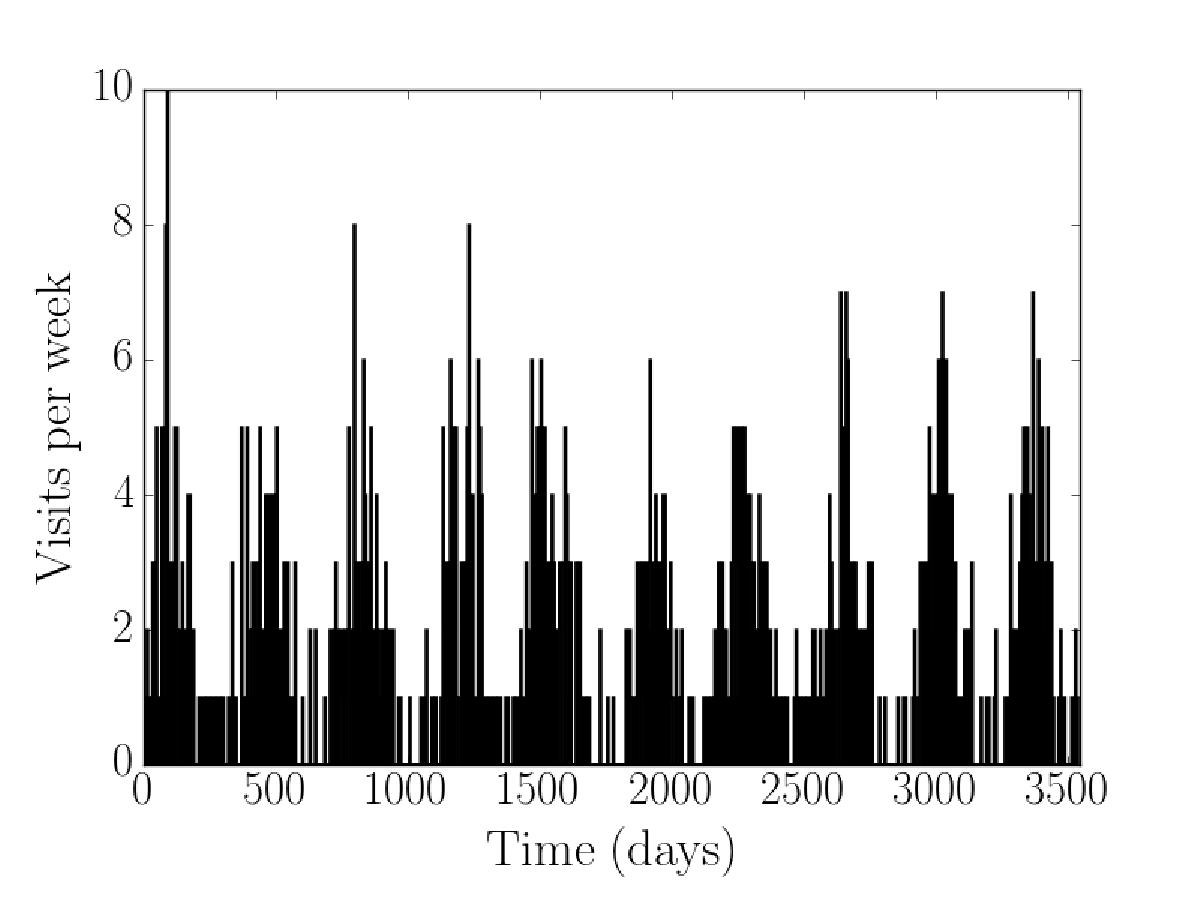
\includegraphics[width=6in, clip=true]{figures/cadence_hist}
\caption[An \LSST\ cadence histogram.]
{A histogram of the number of visits per week as a function of time
for a given object or field observed by \LSST\ as used in our simulations.
Each object is observed only during the day and for half a year at a time.
The code used to generate this plot was written by J. Davenport,
\url{https://github.com/jradavenport/MW-Flare}.}
\label{fig:cadence_hist}
\end{center}
\end{figure}

% \subsection{Field stars}
We used the \TRILEGAL\ \citep{Girardi2012} galaxy simulation code to generate
field stellar populations for five hypothetical \LSST\ fields.
These fields were centred on the same galactic longitude, $l=45$, but
different galactic longitude: $b=-10,-20,-40,-60,-80$.
In this analysis we present results from the $b=-80$ field only, leaving a
more comprehensive study of different stellar populations to future work.
\TRILEGAL\ takes the coordinates and size of a field within the galaxy as
inputs and simulates the population of stars in that field.
It returns a catalogue of simulated stars with their properties: age,
effective temperature and $ugriz$ magnitudes, and others.
We randomly selected 20,000 stars from each field in order to produce a
representative but manageable target sample.
Selected stars had $r$-band magnitudes between 16 and 28 and \logg $>4$.
These target stars were then separated into `cool' ($T_{\mathrm{eff}}< 6250$)
and `hot' ($6250 < T_{\mathrm{eff}}$) temperature bins.
Rotation periods for the cool stars were calculated using the
\citet{Angus2015} gyrochronology relation which converts \TRILEGAL\ ages and
$B-V$ colour (calculated from \TRILEGAL\ $g-r$) into rotation periods.
Hot stars ($T_{\mathrm{eff}}\gtrsim 6250$) lack a significant convective
envelope.
Since the combination of convective plasma motion and stellar rotation is
responsible for magnetic field generation, these stars do not undergo magnetic
braking.
As such, their rotation periods cannot be estimated using gyrochronology.
To assign rotation periods to the hot stars we fitted a sum of two Gaussian
functions to the rotation periods of hot stars in the \citet{Mcquillan2014}
catalogue and randomly sampled from the resulting distribution.
The distribution of hot star rotation periods is shown in figure
\ref{fig:hot_star_hist}.

\begin{figure}
\begin{center}
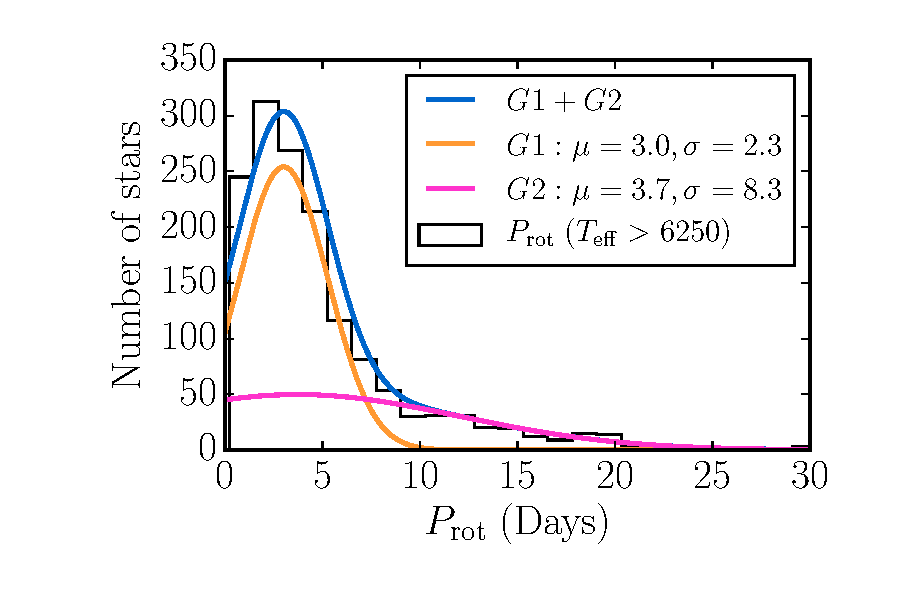
\includegraphics[width=6in, clip=true]{figures/hot_star_hist.pdf}
\caption[A histogram of the rotation periods of hot stars from
\citet{Mcquillan2014}.]
{A histogram of the rotation periods of stars with $T_{\mathrm{eff}} > 6250$K
from the \citet{Mcquillan2014} catalogue.
We fit a sum of two Gaussians to this distribution in order to assign rotation
periods to the hot stars in our \trilegal\ samples.}
\label{fig:hot_star_hist}
\end{center}
\end{figure}

The overall distributions of effective temperatures and theoretical rotation
periods for stars used in our simulations are shown in figures
\ref{fig:trilegal_teff_hist} and \ref{fig:trilegal_period_hist}.
These figures show the distributions for a representative sample of 20,000
stars, randomly selected from the $\sim$ 38,000 total in \trilegal\ field
$l-45$, $b=-80$.

\begin{figure}
\begin{center}
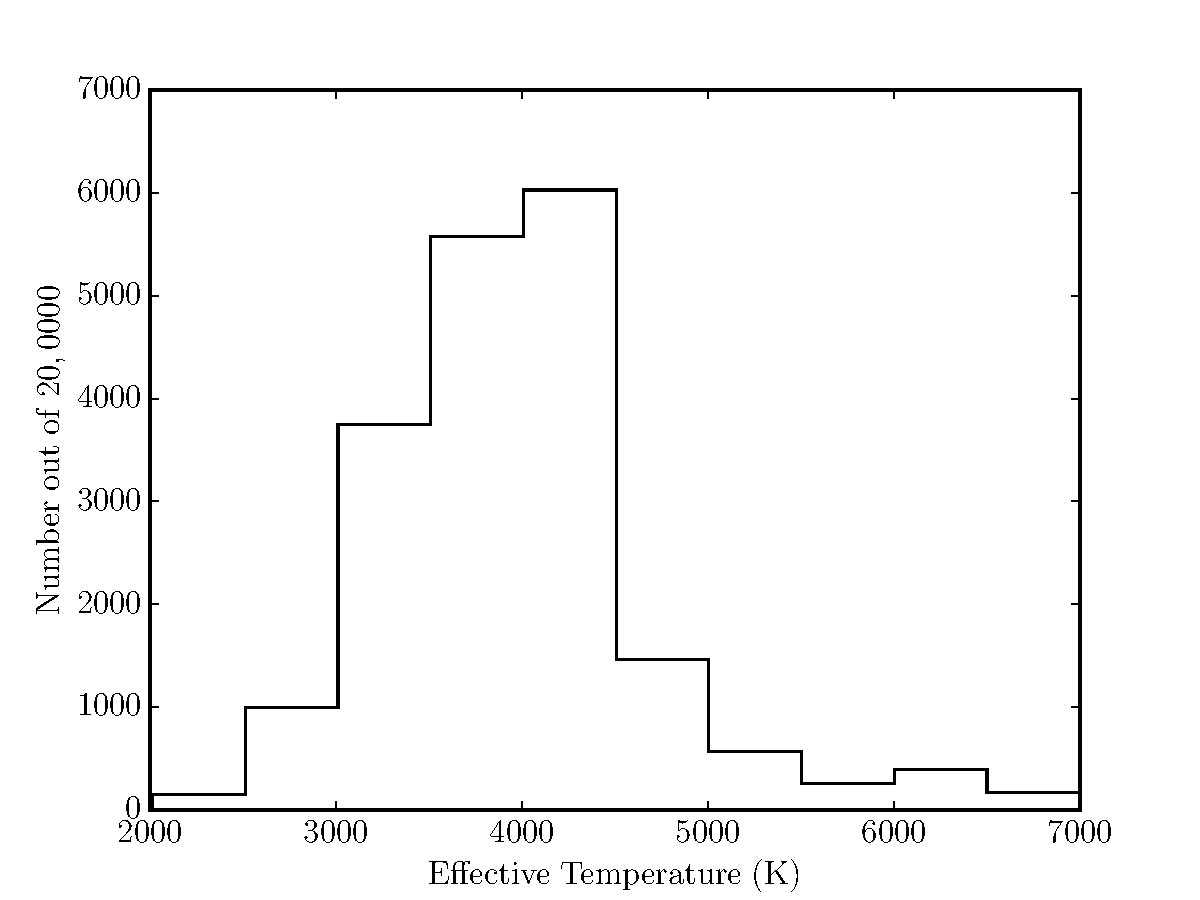
\includegraphics[width=6in, clip=true]{figures/trilegal_teff_hist-80.pdf}
\caption[The effective temperature distribution for stars used in \LSST\
simulations]
{The effective temperature distribution for stars used in our simulations.
We selected 20,000 stars from the $\sim$ 38,000 in the $l=45$, $b=-80$
\trilegal\ field}
\label{fig:trilegal_teff_hist}
\end{center}
\end{figure}

\begin{figure}
\begin{center}
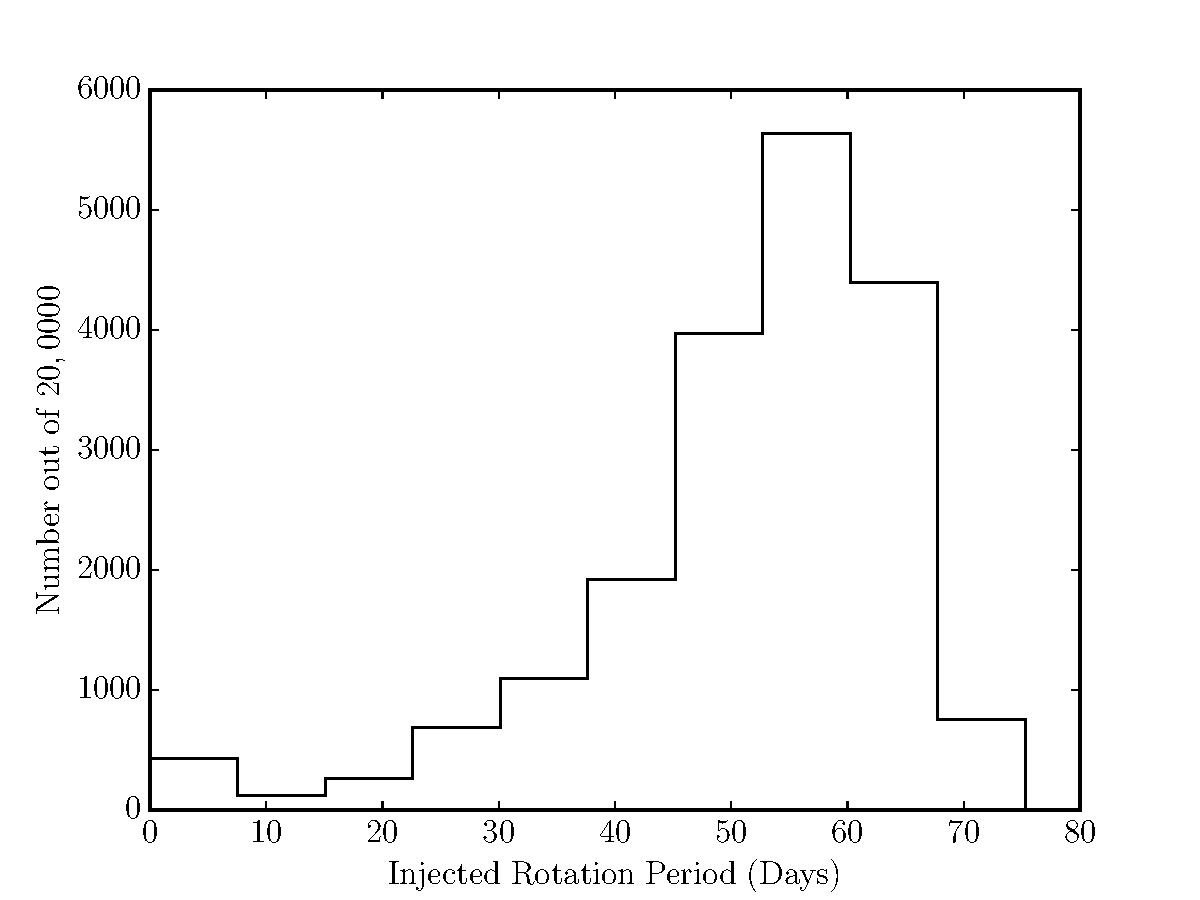
\includegraphics[width=6in, clip=true]{figures/trilegal_period_hist-80.pdf}
\caption[The period distribution for stars used in \LSST\
simulations]
{The distribution of rotation periods used to generate synthetic light curves.
We selected 20,000 stars from the $\sim$ 38,000 in the $l=45$, $b=-80$
\trilegal\ field}
\label{fig:trilegal_period_hist}
\end{center}
\end{figure}

% \subsection{Cluster stars}
% In addition to field stars, we simulated light curves for hypothetical members
% of three open clusters: IC 4651 (1778 Myr), NGC 5316 (170 Myr) and NGC 2477
% (822 Myr).
% Representative numbers of G dwarfs in each cluster were estimated from
% previously published CMDs.
% Numbers of K and M dwarfs were then estimated using the \citet{Kroupa2001}
% initial mass function (IMF).
% Metallicities, distances, reddening, and ages were obtained from the
% \citet{Kharchenko2013} catalogue.
% In order to calculate theoretical rotation periods for stars in these
% clusters, we used three broad temperature bins, corresponding to the three
% spectral types: $G$, $K$ and $M$.
% $G$ type was defined as $5200 < T_{\mathrm{eff}} < 6000$ K, $K$ as $3700 <
% T_{\mathrm{eff}} < 5200$ and $M$ as $2400 < T_{\mathrm{eff}} < 5200$.
% Cluster member catalogues were simulated by randomly drawing effective
% temperatures from uniform distributions bounded by these limits.
% This is a relatively crude way to simulate cluster member temperatures, and an
% improved approach would be to use an IMF.
% We hope to modify our method in future in order to quantify rotation period
% recoverability as a function of effective temperature rather than spectral
% type.
% $B-V$ colours were estimated for cluster members using the
% \citet{Sekiguchi2000} relation for $B-V$, temperature, metallicity and
% \logg\footnote{We used Solar \logg\ for all spectral types.}, and reddening.
% $r$-band magnitudes were then approximated using $B-V$ colour and approximate
% V-band apparent magnitudes for each spectral type in each cluster.
% We generated 2000 each of $G$, $K$ and $M$ dwarfs for all three clusters:
% 18,000 stars in total.
% We simulated equal numbers of G, K and M spectral types, rather than
% representative relative numbers in order to adequately sample the entire
% range of temperature space.
% Using representative numbers would provide excellent M dwarf but very poor G
% dwarf coverage.
% Rotation periods were calculated for the theoretical cluster members using the
% \citet{Angus2015} gyrochronology relation.

\subsection{Synthesising light curves}

Once theoretical rotation periods had been assigned to both hot and cool field
and cluster stars we used code similar to that used in \citet{Aigrain2015b} to
simulate light curves.
These light curves are calculated by placing dark spots on a rotating sphere
and integrating the total resulting flux over the surface.
Stellar flux variations produced by dark active regions on the surface are
typically non-sinusoidal and this simple spot model provides a more accurate
representation of stellar light curves than a simple sinusoid.
However, it should be noted that this code can be adjusted to produce more
realistic light curves by altering spot lifetimes and including differential
rotation with spot migration.
Stars with spot lifetimes that are short relative to their rotation periods
will display quasi-periodic brightness variations in their light curves.
Including differential rotation will compound this effect and further perturb
star spot light curve features from strict periodicity.
We fixed the mean spot lifetime at 30.5 days for all simulations and did not
include differential rotation.
For this reason, our simulated light curves are highly periodic, with only
small deviations from strict periodicity.
Rotation periods are more easy to recover from strictly periodic light curves
than for quasi-periodic ones and for this reason, our results should be
considered `best case'.
In future we plan to vary spot lifetimes and include differential rotation in
our spot model in order to produce more realistic light curves.

In order to assign appropriate amplitudes to the simulated light curves,
the relation between rotation period, amplitude of variability
and \teff was approximated, based on the \citet{Mcquillan2014} sample.
This analysis was performed by collaborator D. Buzasi.
Figure \ref{fig:amp_hist} shows the mean range of variability for stars in
different temperature bins, as a function of their rotation periods.
The range of variability, as defined by \citet{Mcquillan2014} is the
difference between the 5th and 95th percentiles for the fluxes of each data
point in the light curve.
This figure shows that cooler stars have larger variability amplitudes than
cool stars, on average.
It also shows that the variability amplitude declines with rotation period
(or perhaps, age).
The numbers indicated in this figure were used to inform our spot model.
Simulated, \trilegal stars with temperatures and rotation periods falling
within the bins indicated on this plot were assigned amplitudes that were
drawn from Gaussians centred on the mean bin values, with variances that
corresponded to the variance within each bin.

\begin{figure}
\begin{center}
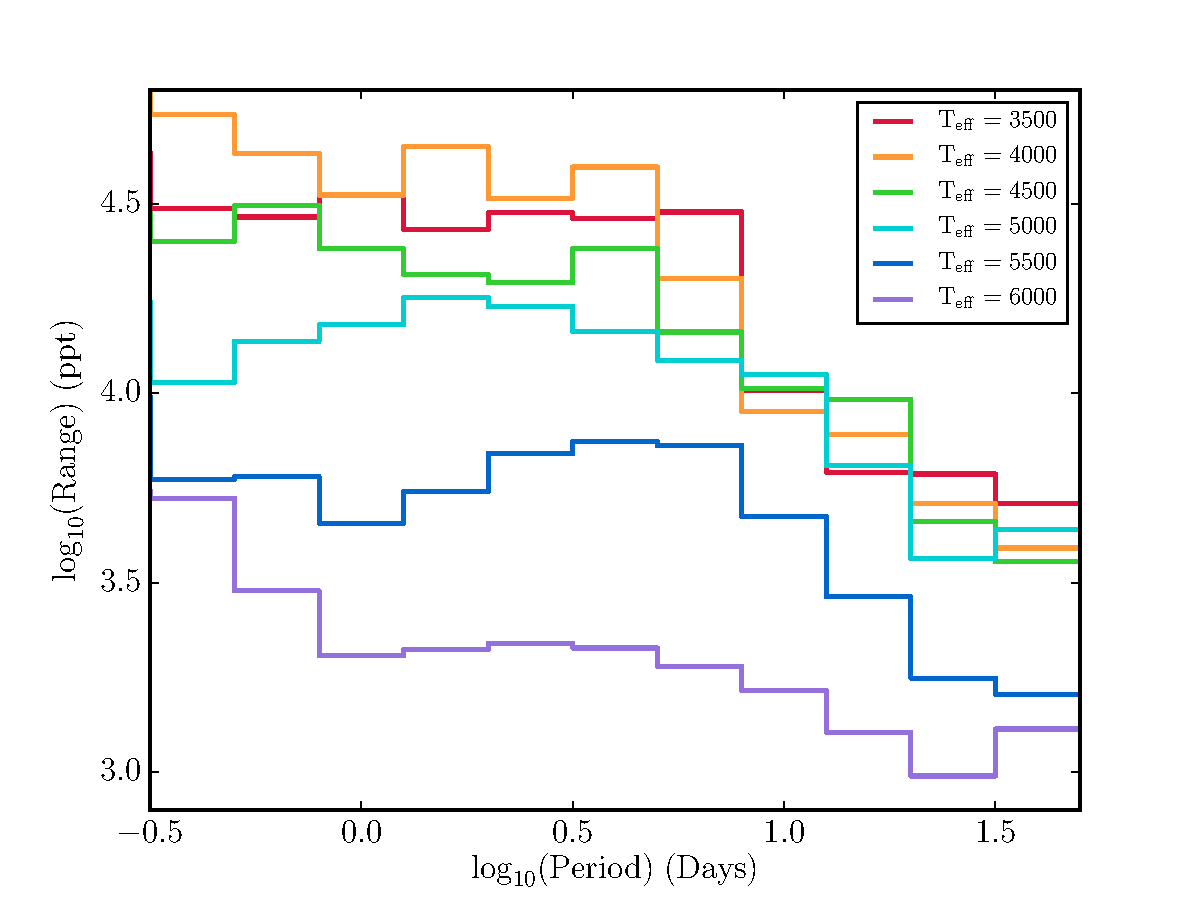
\includegraphics[width=6in, clip=true]{figures/amp_hist.pdf}
\caption[The mean amplitudes of variability for stars in the
\citet{Mcquillan2014} catalogue, according to their temperatures.]
{Mean amplitudes of variability as a function of rotation period, for stars
in the \citet{Mcquillan2014} catalogue.
For each temperature bin indicated, the mean range of variability (the
difference between the 5th and 95th flux percentile) in that bin for all
targets {\it with a measured rotation period} in the \citet{Mcquillan2014} is
plotted as a function of their rotation periods.
These numbers were used to inform our spot model --- stars with temperatures
and rotation periods indicated on this plot were assigned amplitudes
accordingly.
}
\label{fig:amp_hist}
\end{center}
\end{figure}

White noise was added to the light curves, with amplitudes that depended on
$r$-band magnitude, based on the values provided in \citet{Jacklin2015}.
We sampled these light curves using our \LSST\ cadence model and attempted to
recover their rotation periods using a Lomb-Scargle (LS) periodogram
\citep[][]{Lomb1976, Scargle1982}.
LS periodograms were computed for each light curve over a grid of 1000 periods
ranging from 2 to 100 days.
The position of the highest peak in the periodogram was recorded as the
measured period.

As explained previously, a LS periodogram is not ideal for measuring rotation
periods from stellar light curves because star spots tend to produce
non-sinusiodal, quasi-periodic brightness variations.
A commonly used alternative to the LS periodogram is the auto-correlation
function (ACF) which is better suited to non-sinusoidal, quasi-periodic
signals, as demonstrated by \citet{Mcquillan2013}.
Unfortunately however, evenly spaced data are required to produce an ACF.
A comparison of the LS periodogram and ACF methods by \citet{Aigrain2015b}
found good agreement between the two, which is encouraging for this study.
Another alternative method that has produced promising results using Gaussian
processes (GPs) is currently under development \citep{Angus2015b}, however it
is relatively computationally expensive.
We have used the LS periodogram in these initial tests because it is fast to
compute, but intend to use the GP method in the future.

\section{Results}

The results of our simulations are shown in figures \ref{fig:derek} and
\ref{fig:derek2}, where `recovered' rotation periods are plotted against the
`true' rotation periods used to generate the light curves.
Data points are coloured according to their temperatures in figure
\ref{fig:derek} and according to their $r$-band magnitudes in figure
\ref{fig:derek2}.
Rotation periods less than $\sim$ ten days have a low recovery fraction, which
is probably due to the sparcity of \LSST\ sampling.
The large outliers at long rotation periods are mostly faint, as shown in
figure \ref{fig:derek2}.

\begin{figure}
\begin{center}
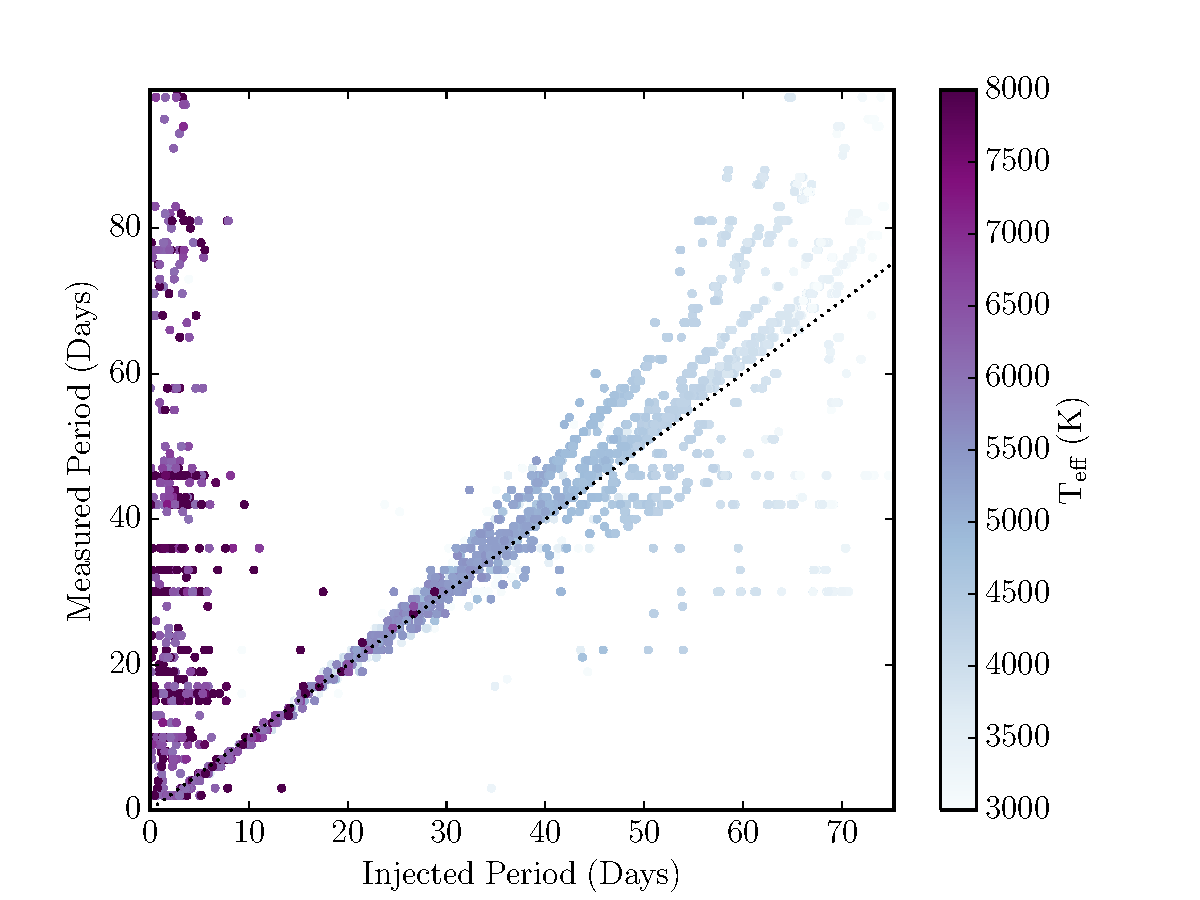
\includegraphics[width=6in, clip=true]{figures/pvp_T_-80.pdf}
\caption[\LSST\ rotation period recovery results with temperature dependence]
{Measured versus injected rotation period for 20,000 simulated \LSST\ targets
in a field centred on $l=-45$, $b=-80$.
Points are coloured according to their temperatures.
Rotation periods less than $\sim$ 10 days have a low recovery fraction, and
this is worse for hot stars as they have lower amplitudes of variability.}
\label{fig:derek}
\end{center}
\end{figure}

\begin{figure}
\begin{center}
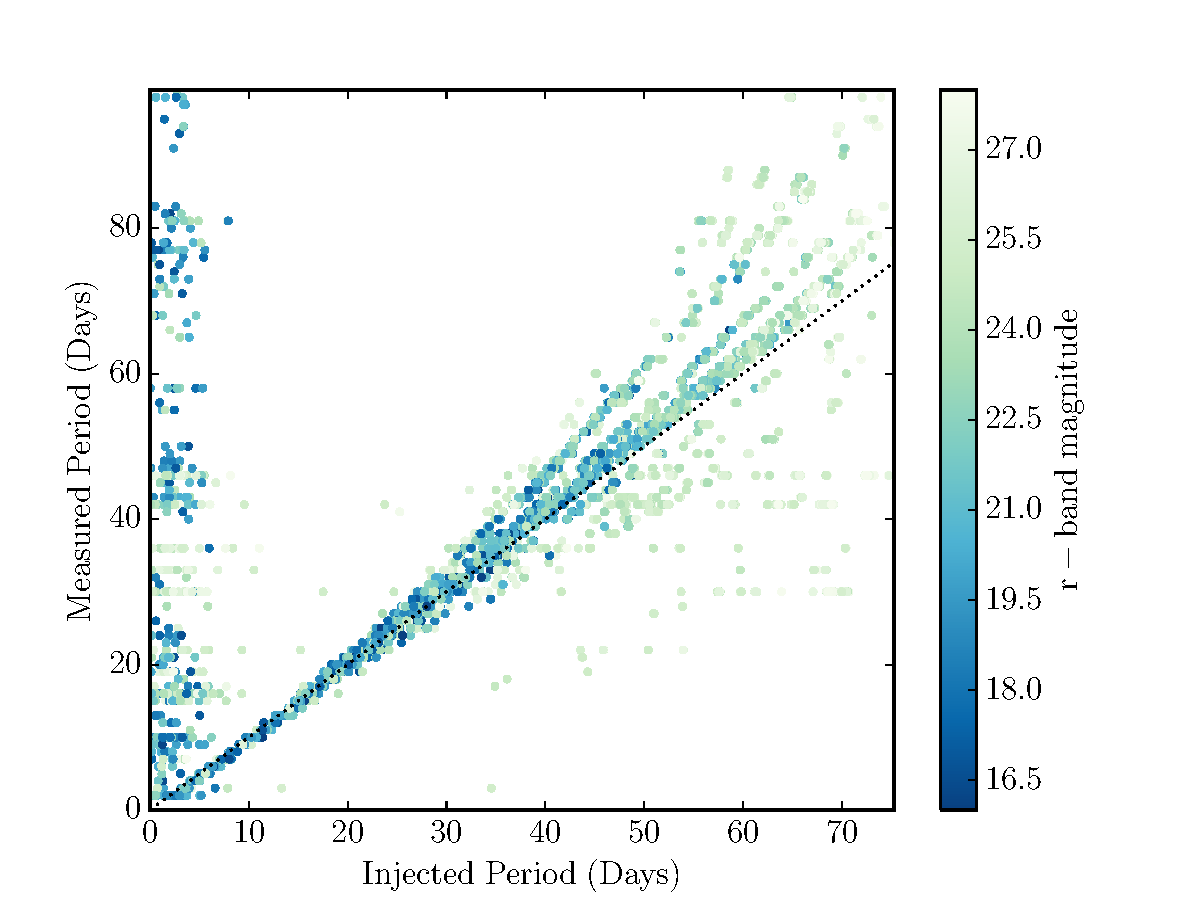
\includegraphics[width=6in, clip=true]{figures/pvp_r_-80.pdf}
\caption[\LSST\ rotation period recovery results with magnitude dependence]
{Measured versus injected rotation period for 20,000 simulated \LSST\ targets
in a field centred on $l=-45$, $b=-80$.
Points are coloured according to the $r$-band magnitude.
The large outliers at long rotation periods are mostly faint.}
\label{fig:derek2}
\end{center}
\end{figure}

The overall fraction of stars with successfully recovered rotation periods
(recovered rotation period lies within 10\% of the injected period) as a
function of input period is shown in figure \ref{fig:kickass}.
The results for $G$ ($5200<\mathrm{T}_{\mathrm{eff}}<6000$), $K$
($3700<\mathrm{T}_{\mathrm{eff}}<5200$), and $M$
($2500<\mathrm{T}_{\mathrm{eff}}<3700$) spectral types are shown separately.
There are no $G$ dwarfs with rotation periods longer than 40 days as these
stars would be older than the galaxy.
This is also the case for $K$ dwarfs with rotation periods greater than 60
days.
For all spectral types, the rotation period sensitivity of \LSST\ peaks at
10-20 days.

\begin{figure}
\begin{center}
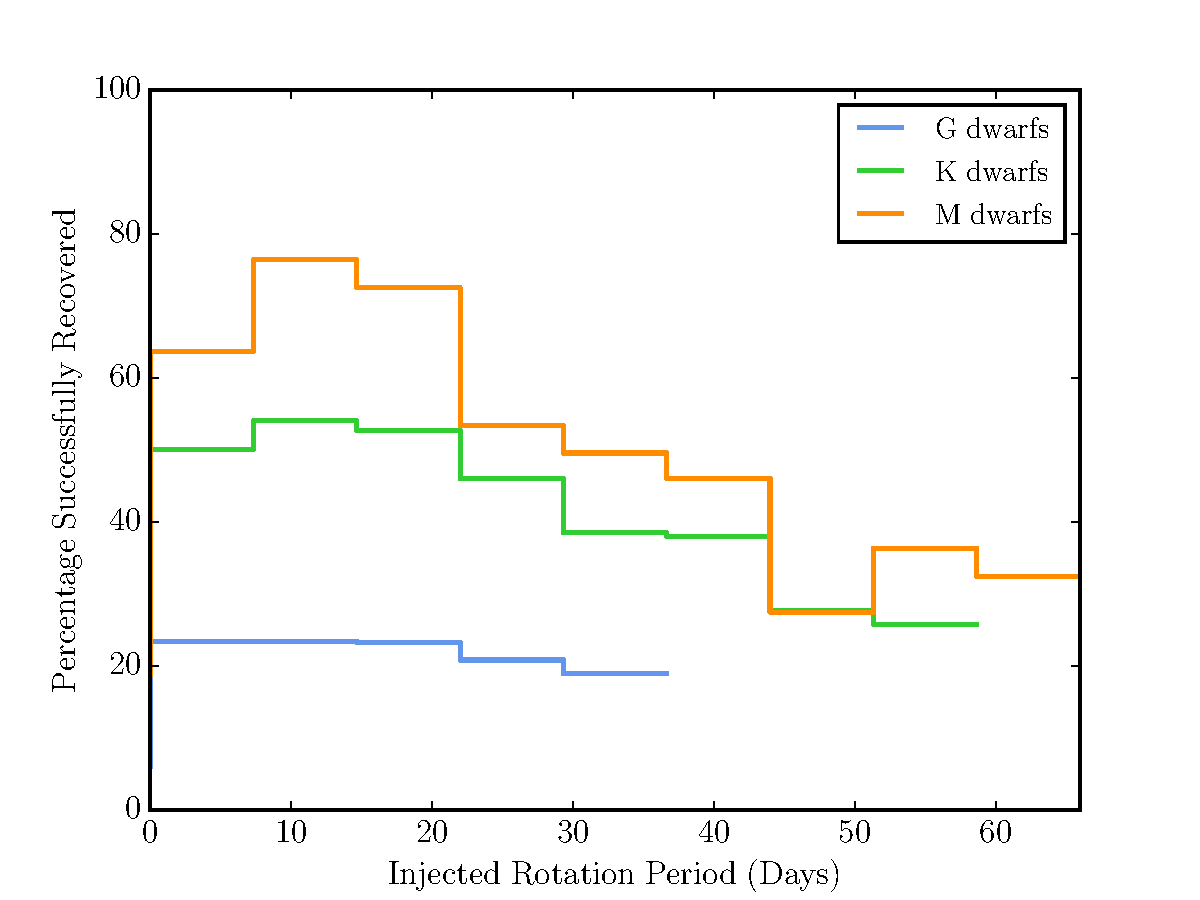
\includegraphics[width=6in, clip=true]{figures/recovered_hist_-10.pdf}
\caption[\LSST\ rotation period recovery results for different spectral types]
{The percentage of successfully recovered rotation periods in each indicated
bin, as a function of input rotation period.}
\label{fig:kickass}
\end{center}
\end{figure}

\section{Conclusions}
Effective temperatures, $r$-band magnitudes, ages and metallicities of 20,000
stars in a hypothetical \LSST\ field (centred on $l=45$, $b=-80$, using the
\trilegal\ stellar population simulation software \citep{Girardi2012}.
Theoretical rotation periods were then calculated for these stars using the
\citep{Angus2015} gyrochronology relation.
Based on the theoretical rotation periods, light curves were simulated for
these stars using a simplified version of the \citep{Aigrain2015} code.
A Lomb-Scargle periodogram was computed for each light curve and a period
measured from the position of the highest peak.
We found that \LSST\ is most sensitive to rotation periods between 10 and 20
days.
Its sensitivity falls at short periods due to the sparcity of its sampling and
at longer periods due to the lower amplitudes of slowly rotating stars.

This work was performed as part of a project to understand the ground-based
optical and infrared follow-up requirements for studying stellar magnetism and
rotation with \LSST.
Going forwards, I intend to expand upon the work presented here by
implementing the improvements listed below.
\begin{itemize}
\item{Using OpSim to generate a more realistic cadence model.}
\item{Using the gyrochronology relation of \citet{Vansaders2013} to
incorporate subgiants into our simulations.
The \citet{Vansaders2013} age-rotation relation applies to subgiants as well
as dwarfs.
Including these stars in our models will provide an indication of the level of
subgiant contamination to expect.}
\item{Using a more realistic spot model.
Our current spot model is overly simplistic and is likely to produce
optimistic results.
Using a model that incorporates differential rotation and variable spot
lifetimes will produce more realistic light curves.}
\item{Applying our method to the whole sky.
The distribution of spectral types and ages varies with galactic coordinate.
Since rotation period recovery success fraction depends on spectral type and
age, this is likely to vary for different fields in the galaxy.}
\item{We would like to investigate the rotation period recovery potential of
the deep drilling fields.
These fields will have much higher cadence and shorter rotation periods are
likely to be detectable within them.}
\end{itemize}
